\documentclass[a4paper,12pt]{article}

\usepackage[utf8]{inputenc}
\usepackage[czech]{babel}
\usepackage[IL2]{fontenc}
\usepackage[left=3cm,text={15cm, 23cm},top=3.5cm]{geometry}

\usepackage{graphicx}
\usepackage{tikz}

\usepackage{amssymb}
\usepackage{amsmath}
\usepackage{amsthm}
\usepackage{forest}
\usepackage[ruled,czech,linesnumbered,noline]{algorithm2e}
\usepackage{array}
\usepackage{multirow}
\usepackage{textcomp}
\usepackage{listings}
\usepackage{multirow}
\usepackage{caption}

\usepackage{xpatch}
\xpretocmd{\algorithm}{\hsize=\linewidth}{}{}
\xpretocmd{\procedure}{\hsize=\linewidth}{}{}

\usepackage{enumitem}
%\usepackage[neverdecrease]{paralist}

\usepackage{pgf}
\usepackage{tikz}
\usetikzlibrary{arrows,automata}

\newcounter{counten}
\setcounter{counten}{1}

\newtheorem{theorem}{Tvrzení}[counten]
\newtheorem{corollary}{Důsledek}[counten]

\lstset{ %
  basicstyle=\footnotesize,
  numbers=left                    % where to put the line-numbers; possible values are (none, left, right)
}


\makeatletter
\newcommand{\dotminus}{\mathbin{\text{\@dotminus}}}

\newcommand{\@dotminus}{%
  \ooalign{\hidewidth\raise1ex\hbox{.}\hidewidth\cr$\m@th-$\cr}%
}
\newcommand{\nosemic}{\renewcommand{\@endalgocfline}{\relax}}% Drop semi-colon ;
\newcommand{\dosemic}{\renewcommand{\@endalgocfline}{\algocf@endline}}% Reinstate semi-colon ;
\newcommand{\pushline}{\Indp}% Indent
\newcommand{\popline}{\Indm\dosemic}% Undent

\makeatother

\begin{document}

\begin{titlepage}

% \vspace*{1cm}
\begin{figure}[!h]
  \centering
  \includegraphics[height=5cm]{img/logo.eps}
\end{figure}

\vfill

\begin{center}
  \bigskip
  \begin{Huge}
  \projname\\
  \end{Huge}
  \begin{large}
  Simulační studie k projektu do předmětu IMS\\
  \end{large}
\end{center}

\vfill

\begin{center}
  \begin{Large}
  \today
  \end{Large}
\end{center}

\vfill

\begin{flushleft}
\begin{large}
\begin{tabular}{ll}
Autor: & \author \\
 & Fakulta Informačních Technologií \\
 & Vysoké Učení Technické v~Brně \\
\end{tabular}
\end{large}
\end{flushleft}
\end{titlepage}


\tableofcontents
\newpage

\section{Úvod}
Tato práce se věnuje optimalizačnímu problému plánování aktivit projektu -- Resource-constrained project scheduling 
problem (dále jen RCPSP). Jedná se o klasický optimalizační problém (\cite{peringer2}, slide 123), který má velké uplatnění i v praxi (generování rozvrhu apod). 
Ačkoliv se jedná o $\mathbf{NP}$-těžký problém, byly již představeny různé druhy heuristik 
pro řešení (genetické algoritmy, simulované žíhání apod.). 
Tato práce se zabývá implementací algoritmu pro řešení RCPSP, který využívá optimalizaci pomocí kolonie mravenců.
Na základě implementovaného nástroje je provedena sada experimentů, které mají ukázat úspěšnost použité metody
a ukázat závislost některých parametrů na kvalitě nalezených řešení.

Autorem této práce je Vojtěch Havlena. Jako hlavní zdroj informací byl zvolen článek \cite{Merkle00antcolony}.
Mimo to bylo ovšem nutné pro sestavení algoritmu a jeho implementaci nastudovat i články \cite{1027745} (rozšíření 
článku \cite{Merkle00antcolony}), \cite{Kolisch1999} a \cite{Blum2005353}, které 
upřesňují a doplňují informace.

\section{Rozbor tématu}
V této kapitole je nejprve definován RCPSP a základní pojmy spojené s tímto problémem. Dále je popsán
základní princip optimalizace pomocí kolonie mravenců, který tvoří základ celé použité metody
pro optimalizaci RCPSP.

\subsection{Formulace problému}
Resource-constrained project scheduling problem (RCPSP) je optimalizační problém plánování aktivit projektu.
Cílem je nalézt takové plánování aktivit, s minimálním rozdílem mezi časem zahájení první aktivity a časem ukončení 
poslední naplánované aktivity, které splňuje omezení kladené na priority mezi aktivitami a omezení na maximální 
využití zdrojů jednotlivých plánovaných aktivit v každém čase.

Formálně je možné RCPSP definovat následovně \cite{Kolisch1999, Merkle00antcolony, 1027745}. Projekt je složen z množiny aktivit $\mathcal{J} = \{0,1,\dots, n+1\}$,
které se mají naplánovat. Aktivity $0$ a $n+1$ odpovídají aktivitám \uv{záhájení projektu} a \uv{ukončení projektu}.
K vykonání aktivity jsou potřeba zdroje, které mají omezenou kapacitu. Celkem je k dispozici $k$ typů zdrojů $\mathcal{K} = \{1, \dots, k\}$ a kapacity 
těchto typů zdrojů jsou určeny množinou kapacit $\mathcal{R} = \{R_1, \dots, R_k\}$, kde $R_i > 0$ je omezení na kapacitu 
zdroje $i \in \mathcal{K}$. Každá aktivita $j\in\mathcal{J}$ má přiřazenu dobu trvání $p_j$ a množství jednotlivý zdrojů $r_{j,k}$, 
kde $k\in\mathcal{K}$ je typ zdroje, požadovaných v každém časovém okamžiku během provádění aktivity $j$.
Předpokládáme, že aktivita 0 a $n+1$ mají dobu trvání $p_j = 0$ a množství zdrojů $r_{j,k} = 0$ pro každé $k\in\mathcal{K}$. 

Kromě omezení
na využití zdrojů, je kladeno také omezení na priority. Pro každou aktivitu $j$ je definována množina jejích předchůdců $\mathcal{P}_j$ 
(aktivita $j$ nemůže být zahájena, před tím, než jsou dokončeny všechny aktivity z $\mathcal{P}_j$).

Rozvrh projektu je reprezentován vektorem $(s_0, s_1, \dots s_{n+1})$, kde $s_j$ je čas zahájení aktivity 
$j\in\mathcal{J}$. Čas ukončení aktivity $i\in\mathcal{J}$ je potom dán jako $f_i = s_i + p_i$. Čas zahájení
projektu je minimum z časů zahájení aktivit, tedy $\min\{s_j\ |\ j\in\mathcal{J}\}$ (odpovídá času $s_0$). Podobně čas ukončení 
projektu je maximum z časů ukončení aktivit, tedy $\max\{f_j\ |\ j\in\mathcal{J}\}$. Makespan je potom rozdíl
mezi časem zahájení a ukončení projektu. 

Rozvrh se nazývá realizovatelný, pokud jsou splněny následující podmínky \cite{Kolisch1999}.
\begin{enumerate}
 \item Aktivita $j\in\mathcal{J}$ nesmí být zahájena před tím, než jsou dokončeny všechny aktivity z $\mathcal{P}_j$ (omezení na priority).
  Tedy $s_j \geq s_i + p_i$, pro každé $i \in \mathcal{P}_j$.
 \item V každém časovém okamžiku $t$ součet požadavků na zdroje naplánovaných aktivit nesmí přesáhnout kapacitu zdrojů.
  Tedy pokud uvažujeme množinu aktivit, které jsou zpracovávány v čase $t$ $A(t) = \{j\in\mathcal{J}\ |\ s_j\leq t < s_j + p_j\}$, tak 
  lze tuto podmínku zapsat jako
  $$
    \sum_{j\in A(t)} r_{j,k} \leq R_k, \mbox{ kde } k\in\mathcal{K}, t \geq 0
  $$
\end{enumerate}
Cílem je potom nalezení realizovatelného rozvrhu pro daný projekt s omezením na zdroje, který má minimální makespan.
V této práci jsou uvažovány pouze single-mode úlohy. U multi-mode úloh je možné vybrat mód úlohy (každý mód využívá jiné
zdroje a má jinou dobu trvání). 

Sady instancí problému RCPS, které jsou uvažovány v této práci jsou dostupné v Project Scheduling Library\footnote{Dostupné na: \texttt{http://www.om-db.wi.tum.de/psplib/main.html}} (PSPLIB). 
Kromě instancí problému jsou zde k dispozici také nejlepší známá řešení pro danou instanci. 

\subsection{Optimalizace pomocí kolonie mravenců}
Optimalizace pomocí kolonie mravenců (ACO) je optimalizační technika, která je inspirována chováním skutečné kolonie mravenců při
shánění potravy. Ve skutečném světě se mravenci zpočátku pohybují prostorem náhodně a v případě nalezení potravy
na zpáteční cestě produkují feromonovou stopu, která určuje vhodnost této cesty. Po této stopě se potom mohou pohybovat další 
mravenci s nadějí, že naleznou další potravu. Nicméně feromonová stopa se postupně vypařuje, což zabraňuje uváznutí v
lokálním optimu \cite{Blum2005353}.

ACO přístup využívá toto chování v přírodě pro řešení optimalizačních problémů. I když existuje mnoho různých variant ACO,
obecně je optimalizační problém pomocí tohoto přístupu řešení opakováním následujících dvou kroků \cite{Blum2005353}.
\begin{itemize}
 \item Pomocí feromonového modelu (\cite{peringer}, slide 7) (parametrizované rozdělení pravděpodobnosti přes celý prostor řešení)(\cite{peringer}, slide 77) a kolonie mravenců jsou
  vytvořena kandidátní řešení.
 \item Kandidátní řešení jsou posléze využity pro úpravu hodnot feromonu.
\end{itemize}
Úpravou hodnot feromonu se docílí toho, že další řešení jsou hledány v okolí již nalezených, kvalitních řešení.
Celé základní schéma algoritmu je uvedeno v algoritmu \ref{alg:aco} \cite{Blum2005353}.

\medskip
\begin{algorithm}[H]
 \SetKwInput{Input}{Input}\SetKwInOut{Output}{Output}
 \SetNlSty{}{}{:}
 \SetNlSkip{-1.2em}
 \SetInd{1em}{1em}
 \BlankLine
 \Indentp{1.7em}
     \While{$\mathbf{not}$ $kriterium\_zastaveni$} {
	Pomocí mravenců vytvoř řešení \\
	Aktualizuj hodnoty feromonů \\
	Proveď centralizované akce \\
     }
 \caption{\textsc{Schéma ACO}}
 \label{alg:aco}
\end{algorithm}

\medskip
\emph{Pozn.} Centralizované akce jsou akce, které nemohou být provedeny jednotlivými mravenci (lokální optimalizace, sběr globálních dat, \dots).

\section{Abstraktní koncepce práce}

Jádrem celé procedury pro heuristické řešení RCPSP je schéma generování rozvrhu (GS). GS buduje realizovatelný
rozvrh postupným rozšiřováním částečného rozvrhu, který vznikl v daném kroku GS. Částečný rozvrh je rozvrh ve kterém je 
naplánována pouze podmnožina aktivit. V článku \cite{Merkle00antcolony} (i v mé implementaci)
je použito sériové schéma generování rozvrhu (článek \cite{1027745} obsahuje implementaci i paralelního schématu, ten
zde však není uvažován).

\subsection{Sériové schéma generování rozvrhu}
Sériové schéma generování rozvrhu (SGS) vytváří realizovatelný rozvrh z částečného rozvrhu, který na počátku obsahuje pouze aktivitu $0$ 
naplánovanou na čas $0$. SGS potom pracuje v $n$ krocích a každém kroku je vybrána jedna aktivita a ta je 
naplánována na nejnižší čas, tak aby byly splněny omezení na priority a zdroje.
Je známo, že pro každou instanci RCPSP je možné nalézt optimální řešení pomocí SGS \cite{Kolisch1999}. V SGS jsou v každém kroku $g = 1,\dots,n$ využívány 
následující množiny \cite{Kolisch1999}. 
\begin{itemize}
 \item Množina $\mathcal{S}_g$ obsahuje již naplánované aktivity.
 \item Množina vhodných aktivit $\mathcal{D}_g$ obsahuje aktivity, které je možné aktuálně naplánovat. V této množině
  jsou aktivity, které ještě nebyly zařazeny do rozvrhu a všichni předchůdci již byli naplánováni, 
    $\mathcal{D}_g = \{ j\in\mathcal{J}\setminus\mathcal{S}_g\ |\ \mathcal{P}_j\subseteq \mathcal{S}_g \}$.
 \item Zbývající kapacita zdroje typu $k$ v čase $t$ $\tilde{R}_k(t) = R_k - \sum_{j\in A(t)} r_{j,k}$.
 \item Množina všech časů dokončení aktivit $\mathcal{F}_g = \{f_j\ |\ j \in\mathcal{S}_g\}$.
\end{itemize}
Zápis v pseudokódu potom vypadá následovně \cite{Kolisch1999, 1027745}.

\medskip
\begin{algorithm}[H]
 \SetKwInput{Input}{Input}\SetKwInOut{Output}{Output}
 \SetNlSty{}{}{:}
 \SetNlSkip{-1.2em}
 \SetInd{1em}{1em}
 \Input{Instance RCPSP}
 \Output{Realizovatelný rozvrh}
 \BlankLine
 \Indentp{1.7em}
    $F_0 = 0$, $\mathcal{S}_0 = \{ 0 \}$ \\
    \For{$g = 1$ to $n$} {
      Vypočítej $\mathcal{D}_g$, $\mathcal{F}_g$, $\tilde{R}_k(t)$ pro $k\in\mathcal{K}$ a $t\in \mathcal{F}_g$ \\
      Vyber aktivitu $j\in\mathcal{D}_g$ \\
      $EF_j = \max_{h \in \mathcal{P}_j}\{ f_h \} + p_j$ \\
      \nosemic $f_j = \min\big\{ t\in [EF_j - p_j, LF_j - p_j] \cap \mathcal{F}_g\ |\ r_{j,k}\leq \tilde{R}_k(\tau),$ \;
	\pushline\dosemic $k \in\mathcal{K}, \tau\in [t,t+p_j[\,\cap\, \mathcal{F}_g \big\} + p_j$ \\
      \Indm $\mathcal{S}_g = \mathcal{S}_{g-1}\cup \{ j \}$
    }
    $f_{n+1}  = \max_{h \in \mathcal{P}_{n+1}}\{ f_h \}$
 \caption{\textsc{Sériové schéma generování rozvrhu}}
 \label{fastSlam}
\end{algorithm}

\medskip
Na začátku každé iterace jsou nejprve spočítány množiny $\mathcal{D}_g$, $\mathcal{F}_g$ a $\tilde{R}_k(t)$
pro $t \in \mathcal{F}_g$. V dalším kroku je vybrána jedna aktivita $j$ z množiny vhodných aktivit.
V případě článků \cite{Merkle00antcolony, 1027745} se k výběru vhodné aktivity používá optimalizace pomocí kolonie mravenců, což
je podrobněji popsáno v dalších podkapitolách.
Po výběru aktivity $j$ je spočítána hodnota $EF_j$ (earliest finish time), což je maximum z časů ukončení všech předchůdů 
aktivity $j$ plus doba trvání $j$. Pro výpočet času ukončení $f_j$ je také nutné znát hodnotu $LF_j$ (latest finish time),
která může být rekurzivně spočítána následovně \cite{1027745, DBLP:journals/jcp/LiuY11a}:
\begin{eqnarray*}
  LS_{n+1} &=& LF_{n+1} = T_{max}\\
  LF_j &=& \min\{LS_i\ |\ i\in\tilde{\mathcal{S}}_j\},\quad LS_j = LF_j - p_j,\mbox{ pro }j = n,\dots, 0,
\end{eqnarray*}
kde $\tilde{\mathcal{S}}_j$ je množina přímých následovníků aktivity $j$ (podle omezení na priority) a $T_{max}$ je 
horní omezení času ukončení projektu. 

\subsection{Využití ACO pro generování rozvrhu}
Jak již bylo zmíněno dříve, optimalizace pomocí kolonie mravenců (ACO) je využita pro rozhodnutí, která
aktivita z množiny vhodných aktivit bude vybrána v každém kroce SGS.
ACO algoritmus použitý v článcích \cite{1027745, Merkle00antcolony} pracuje tak, že v každé generaci, každý z $m$ mravenců v populaci
vytvoří jedno řešení pomocí SGS. Pro výběr aktivity z množiny vhodných aktivit se využívá feromonová
a heuristická informace. Feromonová informace $\tau_{ij}$ a heuristická informace $\eta_{ij}$ udávají,
jak vhodné se zdá být napánovat aktivitu $j$ jako $i$-tou v SGS (v $i$-té iteraci). Feromonová informace
pochází od mravenců, kteří dříve nalezli dobrá řešení (vzhledem k hodnotě makespan projektu).

Aktivita z množiny vhodných aktivit je vybrána podle pravděpodobnostního rozložení přes 
množinu vhodných aktivit $\mathcal{D}$ v dané iteraci SGS, které je určeno následujícím
vztahem \cite{1027745, Merkle00antcolony}:
\begin{equation}
  p_{ij} = \frac{[\tau_{ij}]^\alpha[\eta_{ij}]^\beta}{\sum_{h\in\mathcal{D}}[\tau_{ih}]^\alpha[\eta_{ih}]^\beta},
\end{equation}
kde $\alpha$ a $\beta$ jsou konstantní hodnoty, které určují relativní vliv feromonové a heuristické
informace na výběr aktivity. 

Jako heuristická informace $\eta_{ij}$ je použita LFT heuristika (latest finish time),
která plánuje aktivity podle rostoucí hodnoty $LF$ \cite{1027745, Merkle00antcolony}. Heuristika využívá toho, že relativní rozdíly mezi hodnotami
$LF$ pro aktivity, které se stanou vhodné pro plánování až později, jsou obvykle malé. Proto se používá 
rozdíl mezi maximem hodnot $LF$ z aktivit, které jsou v množině vhodných aktivit a hodnotou $LF_j$ dané aktivity $j$.
Hodnotu $\eta_{ij}$ lze tedy spočítat následovně \cite{1027745, Merkle00antcolony}:
\begin{equation}
 \eta_{ij} = \max_{k\in\mathcal{D}} LF_k - LF_j + 1
\end{equation}

Na konci každé generace ACO algoritmu dochází ke změně feromonové informace -- aktualizuje se feromonová matice.
Nejprve se feromonová matice aktualizuje podle vztahu \cite{1027745, Merkle00antcolony}:
$$
  \tau_{ij} = (1-\rho)\cdot\tau_{ij},
$$
kde parametr $\rho$ udává míru vypařování feromonu. Celý tento vztah reprezentuje postupné vypařování feromonu.
Dále je feromonová matice aktualizována podle nejlep\-šího nalezeného řešení v aktuální generaci algoritmu a nejlepšího
dosud nalezeného řešení (ze všech generací). Tato strategie má za následek prohledávání v okolí dříve nalezených 
nejlepších řešení. Tedy pro každou aktivitu $j\in\mathcal{J}$, která byla v nejlepším dosud nalezeném řešení umístěna na pozici $i$ 
(vybrána jako $i$-tá v SGS), je hodnota $\tau_{ij}$ upravena následovně \cite{1027745, Merkle00antcolony}:
$$
  \tau_{ij} = \tau_{ij} + \rho\cdot\frac{1}{2T^*},
$$
kde $T^*$ je makespan nejlepšího dosud nalezeného řešení. Stejný postup je aplikován i na nejlepší řešení, které
bylo nalezeno v aktuální generaci. 
Celé základní schéma základního algoritmu lze tedy zapsat následovně.

\medskip
\begin{algorithm}[H]
 \SetKwInput{Input}{Input}\SetKwInOut{Output}{Output}
 \SetNlSty{}{}{:}
 \SetNlSkip{-1.2em}
 \SetInd{1em}{1em}
 \Input{Instance RCPSP}
 \Output{Realizovatelný rozvrh}
 \BlankLine
 \Indentp{1.7em}
    Inicializace $\tau_{ij}, \eta_{ij}$ \\
%    $bestGen = \emptyset$, $bestSoFar = \emptyset$ \\
    \While{$\mathbf{not}$ $kriterium\_zastaveni$} {
%      $bestGen = \emptyset$ \\
      \For{$i = 1$ to $m$} {
	 Nalezni řešení $sol$ pomocí SGS s aktuálními hodnotami $\tau_{ij}, \eta_{ij}$ \\
	 Aktualizuj nejlepší řešení nalazené v aktuální generaci.
      }
      Aktualizuj dosud nejlepší nalazené řešení.\\
      Aktualizuj hodnoty $\tau_{ij}$
    }
 \caption{\textsc{Základní schéma algoritmu}}
 \label{fastSlam}
\end{algorithm}

\medskip
Nejprve je provedena inicializace hodnot $\tau_{ij}, \eta_{ij}$. Hlavní cyklus ACO algoritmu se provádí dokud 
není splněno kritérium zastavení, což je zde, dokud není proveden určitý maximální počet generací. V cyklu
dále každý mravenec z celkové populace $m$ mravenců vytvoří řešení pomocí SGS. SGS je stejné, jak bylo
popsáno v předchozí podkapitole, pouze s tím rozdílem, že výběr aktivity $j$ z množiny vhodných aktivit
se provede s pravděpodobností, která je určena pomocí (1). Nakonec se pouze aktualizují hodnoty $\tau_{ij}$
podle míry odpařování a podle nalazených nejlepších řešení.

\subsection{Použité heuristiky}
V této podkapitole jsou popsány další použité heuristiky, které byly zmíněny v článcích \cite{Merkle00antcolony, 1027745} a posléze naimplementovány.

\subsubsection{Kombinace přímého a souhrnného vyhodnocení}
Vyhodnocení hodnoty $p_{ij}$, tak jak bylo popsáno ve vztahu (1) se nazývá příme vyhodnocení. Mimo toto existuje
také souhrnné vyhodnocení, které je dáno následovně~\cite{Merkle00antcolony}:
\begin{equation}
  p_{ij} = \frac{(\sum_{k=1}^i[\tau_{kj}])^\alpha[\eta_{ij}]^\beta}{\sum_{h\in\mathcal{D}}(\sum_{k=1}^i[\tau_{kh}])^\alpha[\eta_{ih}]^\beta}
\end{equation}
Místo, aby se použilo pouze přímé vyhodnocení nebo pouze sourhnné vyhodnocení, použije se v algoritmu 
jejich kombinace, která se získá následovně. V článku je využit parametr $c$, který určuje relativní
vliv přímého a souhrnného vyhodnocení. Pravděpodobnostní rozložení, které se využívá pro výběr další
aktivity je spočítána jako ve vztahu (1), ale s tím rozdílem, že hodnoty $\tau_{ij}$ jsou nahrazeny
za hodnoty $\tau'_{ij}$, které jsou vypočítány jako \cite{Merkle00antcolony}
$$
  \tau'_{ij} = c\cdot x_i\cdot\tau_{ij} + (1-c)\cdot y_i\cdot\sum_{k = 1}^i\tau_{kj},
$$
kde hodnoty $x_i = \sum_{h\in\mathcal{D}}\sum_{k = 1}^i\tau_{kh}$ a $y_i = \sum_{h\in\mathcal{D}}\tau_{ih}$
upravují vliv přímého a souhrnného vyhodnocení (v článku \cite{1027745} navíc v uvedeném vztahu vystupuje
parametr $\gamma$, který zde ale není uvažován, tj. $\gamma = 1$, stejně jako v \cite{Merkle00antcolony}).

\subsubsection{Lokální optimalizační strategie}
Další použitou heuristikou je použití lokální optimalizační strategie. Lokální optimalizační strategie
je použita na řešení, která byla nalezena kolonií mravenců. Takto použitá optimalizační strategie
může ještě vylepšit nalezená řešení \cite{Merkle00antcolony, 1027745}.

Pro vylepšení nalezeného řešení je použita 2-opt strategie. Tato strategie spočívá ve výměnách
mezi dvojicemi aktivit v nalezeném řešení. Pro každou dvojici aktivit $(i,j)$, kde $i < j$ se
provede prohození aktivity $i$ a $j$ v aktuálním řešení a pomocí modifikovaného SGS se na základě změněného 
řešení provede nové plánování. 
Modifikace SGS spočívá v tom, že z množiny vhodných aktivit se vybere ta, která je v předaném řešení 
na daném místě (tedy pořadí výběru a plánování aktivit je dáno změněným řešením).
Pokud
je nově naplánovaný rozvrh realizovatelný a je lepší (má menší makespan) než řešení, kde 
aktivity $i$ a $j$ nejsou prohozeny, je aktuální řešení nahrazeno za nové a další výměny jsou
prováděny již na něm.

Strategie 2-opt je výpočetně velmi náročná, proto ji není vhodné používat na každé řešení, které
bylo v dané generaci nalezeno, ale například na nejlepší nalezené řešení v rámci jedné generace.
Je rovněž možné použít modifikovanou verzi, která
uvažuje výměny aktivit v řešení s indexy $i,j$, $i < j$.

\subsubsection{Zapomínání nejlepších řešení}
Vzhledem k tomu, jakým způsobem je upravována feromonová informace $\tau_{ij}$, nejlepší
nalezené řešení, které je stabilní (zůstává nejlepším) po mnoho generací, má 
velký vliv na feromonovou informaci. Může se tedy stát, že všechna řešení získaná v 
dané generaci budou postupně konvergovat k tomuto nejlepšímu řešení a algoritmus
uvázne v lokálním minimu. Aby se předešlo tomuto problému je s malou pravděpodobností
$p_w > 0$ nejlepší dosud nalezené řešení nahrazeno nejlepším řešením, které bylo 
získáno v dané generaci (i když je horší než nejlepší dosud nalezené řešení) \cite{Merkle00antcolony, 1027745}.

\section{Popis implementace}
Tato kapitola je věnována samotnému popisu implementace simulačního modelu (\cite{peringer}, slide 44). Základem je algoritmus pro řešení RCPSP pomocí
ACO, který byl popsán v předchozí kapitole. Celý program byl napsán v jazyce Python (verze 2.7.9) a 
na nejvyšší úrovni je složen z několika tříd:
\begin{itemize}
 \item Třída \texttt{Job} reprezentuje aktivitu RCPSP. Ve třídě jsou uloženy informace
  o číslu aktivity, době tvání, požadovaných zdrojích, času ukončení a informace
  o bezprostředních předchůdcích a následovnících (plyne z omezení na priority).
 \item Třída \texttt{InputParser} slouží k parsování vstupního souboru, který obsahuje
  instanci RCPSP. Předpokládá se, že soubor je zadán ve formátu, který je 
  použit v knihovně PSPLIB (soubory s příponou .sm).
 \item Třída \texttt{SerialScheduleLocalOpt} implementuje lokální optimalizační strategii
  2-opt, která byla popsána v podkapitole 2.3.2.
 \item Třída \texttt{SerialSchedule} obsahuje implementaci sériového schématu generování
 rozvrhu.
 \item Třída \texttt{SolutionValidity} je třída, která pro nalezené řešení zkontroluje, zda
  je toto řešení opravdu realizovatelné (využito pro účely ladění).
 \item Třída \texttt{CriticalPath} zajišťuje pro zadanou instanci RCPSP výpočet dolního ohraničení kritické cesty.
  Dolní ohraničení kritické cesty je nejdelší cesta v grafu aktivit instance RCPSP (aktivity jsou uzly, 
  předchůdci definují hrany a doba trvání aktivity je ohodnocení hrany). 
  Pro vypočítání této hodnoty jsou nejprve uzly grafu aktivit topologicky uspořádány.
  Následně se s využitím uspořádaných uzlů spočítá nejdelší cesta v grafu, což je hledaná
  hodnota.
\end{itemize}
Tyto zmíněné třídy jsou využity v hlavní funkci programu -- \texttt{AntCycle}, která 
implementuje základní schéma algoritmu 2. Nyní se blíže podíváme na implementaci 
hlavních částí celého algoritmu pro RCPSP.

\subsection{Implementace sériového schéma generování rozvrhu}
Jak již bylo zmíněno dříve, sériové schéma generování rozvrhu je implementováno
ve třídě \texttt{SerialSchedule}, konkrétněji v metodě \texttt{ProcessScheme}. Výpočet probíhá v cyklu, stejně, jak je uvedeno
v algoritmu 2. V každé iteraci je nejprve spočítána množina vhodných aktivit (metoda \texttt{EligibleSet} a množina časů ukončení
již naplánovaných aktivit (metoda \texttt{FinishTimes}). V celé implementaci je hojně
využíván vestavěný datový typ \texttt{set}, který reprezentuje množinu a poskytuje efektivní implementaci
množinových operací. 

V dalším kroku je s využitím LFT heuristiky aktualizována hodnota 
$\eta_{ij}$ (podle vztahu (2)). K výpočtu této hodnoty je ale potřeba znát hodnotu $LF_j$, kterou
ovšem není třeba počítat znovu v každé iteraci, proto je hodnota $LF_j$ pro všechny $j\in\mathcal{J}$
spočítána jednou ještě před samotným SSG algoritmem.

Následně je podle spočítané hodnoty $\eta_{ij}$ a aktuální hodnoty $\tau_{ij}$. vybrána jedna aktivita
z množiny vhodných aktivit (metoda \texttt{ChooseFromElSet}. Toto je provedeno pomocí heuristiky kombinace 
přímého a souhrnného vyhodnocení (viz. podkapitola 3.3.1).

Poté je zjištěna hodnota $EF$ zvolené aktivity a následně je spočítán čas ukončení
této zvolené aktivity (metoda \texttt{Finish}). Metoda \texttt{Finish} počítá zbývající
kapacitu naplánovaných aktivit v jednotlivých časech a zvolenou aktivitu zařadí na nejnižší čas, 
ve kterém je dostatek zdrojů. Pro výpočet zbyvající kapacity v daných časech slouží
metoda \texttt{RemainingCapacities}. Provádění metody \texttt{Finish} se ukázalo jako
výpočetně nejnáročnější ze všech operací prováděných v jedné iteraci SSG  (právě kvůli 
opakovanému výpočtu zbývajících kapacit). Aby výpočet nebyl příliž dlouhý, bylo tedy nutné
provést optimalizaci, která je popsána dále.

Nakonec se jen vybraná aktivita se spočítaným časem ukončení vloží do množiny naplánovaných aktivit.

\subsubsection{Optimalizace metody Finish}

Optimalizace spočívá v ukládání zbývajících kapacit v jednotlivých časech
do asociativního pole. Klasické pole nebylo využito, protože i když přístup k jednotlivým
prvkům je rychlejší než v případě asociativního pole, tak kvůli nutnosti inicializace klasického pole na počátku SGS,
byla implementace pomocí klasického pole pomalejší než pomocí asoc. pole.

Byla také zkoušena varianta, kdy se do asoc. pole ukládala informace, jaká aktivita je v
kterém čase aktivní. Pomocí této informace se potom počítala zbývající kapacita v daném
čase. Nicméně provedené experimenty ukázaly, že ukládání zbývajících kapacit v jednotlivých časech
je efektivnější než ukládání aktivních aktivit.

Aby optimalizace pomocí asoc. pole správně fungovala, je nutné informaci v poli aktualizovat po každém
vložení aktivity do rozvrhu (na konci každé iterace SGS).

\subsection{Implementace lokální optimalizační strategie}

Lokální optimalizační strategie 2-opt, jak je popsána v podkapitole 3.3.2 je implementována
ve třídě \texttt{SerialScheduleLocalOpt} (odvozena od třídy \texttt{SerialSchedule}), konkrétně v metodě \texttt{LocalOptimisationStrategy}.
Parametrem této metody je nalezené realizovatelné řešení, které se má optimalizovat. Tato
metoda postupně prohazuje aktivity $i,j,i<j$ a aplikuje na ně metodu 
\texttt{OptSSGS}. Byla naimplementována i výměna aktivit s indexy $i$ a $j$, $i<j$ v řešení, nicméně se ukázalo, že výměna na 
úrovni aktivit dává mírně lepší výsledky. Pokud řešení vzniklé metodou \texttt{OptSSGS} je lepší než stávající
nejlepší řešení, je stávající řešení nahrazeno za nově vzniklé a náhrady jsou dále prováděny
s tímto řešením.

Metoda \texttt{OptSSGS} implementuje speciální případ SGS, kdy výběr aktivity do rozvrhu
z množiny vhodných aktivit je určen řešením, které je předáno jako argument. Není
zde tedy třeba porovádět aktualizaci hodnot $\eta_{ij}$ a ani volat funkci 
\texttt{ChooseFromElSet}. Pouze se pro aktivitu spočítá nový čas ukončení (metoda \texttt{Finish}).
Aplikace lokální optimalizační strategie je výpočetně velmi náročné, proto bylo
nutné opět provést určité optimalizace jako je redukce počtu volání metody \texttt{OptSSGS}.

\subsubsection{Redukce počtu volání OptSSGS}
Vzhledem k výpočetní složitosti metody \texttt{OptSSGS}, bylo nutné redukovat počet volání této metody.
Při prohození dvou aktivit v řešení se může stát, že nové řešení již nebude realizovatelné (což je 
následně odhaleno v metodě \texttt{OptSSGS}). Pro urychlení celého procesu se před zavoláním \texttt{OptSSGS}
provede rychlá kontrola, která odfiltruje některá nerealizovatelná řešení. Tato kontrola se provádí
v metodě \texttt{CanSwap}, která využívá pro každou aktivitu předem vypočítanou informaci o množině 
všech předchůdců. Na základě toho lze odfiltrovat řešení, která porušují podmínku priority a tedy
redukovat počet volání metody \texttt{OptSSGS}.

\subsection{Implementace celého algoritmu}
Hlavní funkcí programu je funkce \texttt{AntCycle}, která implementuje celý ACO algoritmus. 
Tato funkce obsahuje cyklus, kdy jedna iterace odpovídá jedné generaci algoritmu. V každé
generaci, každý z $m$ mravenců nalezne jedno řešení pomocí SGS (metoda \texttt{ProcessScheme}).
Na nejlepší nalezené řešení v dané generaci se potom aplikuje lokální opt. strategie 
(metoda \texttt{SerialScheduleLocalOpt}). Nicméně kvůli výpočetní složitosti opt. strategie
může být použití omezeno na každou $n$-tou generaci (záleží na parametru). Následně je 
podle nejlepších řešení aktualizována hodnota $\tau_{ij}$ a s určitou malou pravděpodobností
je dosud nejlepší řešení nahrazeno nejlepším řešením dané generace (heuristika zapomínání
nejlepšího řešení). Stručný manuál k programu je uveden v příloze A.

\section{Provedené experimenty}
Cílem experimentování je zjistit, jak kvalitní řešení (vzhledem k hodnotě makespan rozvrhu) lze 
pomocí naimplementovaného nástroje nalézt pro zadanou sadu instancí RCPSP. Kromě toho také
zjistit, jak závisí kvalita nalezeného rozvrhu na hodnotě některých parametrů.

Jako množina vstupních testovacích instancí byla zvolena množina instancí, která je dostupná
z knihovny PSPLIB. Knihovna obsahuje velké množství instancí problému, které jsou rozděleny do sad podle
celkového počtu aktivit v instanci (30, 60, 90 a 120 aktivit). Každá sada obsahuje instance problémů,
které byly vygenerovány s využitím různých parametrů (průměrný počet předchůdců, omezenost zdrojů, \dots).
Pro každou instanci problému je v knihovně také k dispozici makespan optimálního, resp. heuristického řešení.

Vyhodnocování experimentu potom spočívá ve výpočtu průměrné odchylky od optimálního/heuristického řešení.
Pro sadu j120 byla také počítána odchylka od dolního ohraničení kritické cesty (lower bound critical path, LB CP).

V dílčích experimentech je pomocí $c$-RCPSP-LO označen algoritmus popsaný v kapitole 3, který navíc
obsahuje všechny popsané heuristiky (zapomínání nejlepších řešení, kombinace přímého a souhrnného vyhodnocení s parametrem $c$ a
lokální opt. strategii) a $c$-RCPSP označuje algoritmus, kde není využita lok. opt. strategie (jinak 
je stejný jako $c$-RCPSP-LO). Vzhledem k výpočetní náročnosti lokální optimalizace se neprovádí
každou iteraci, ale pouze každou dvacátou iteraci.

\subsection{Experiment 1 -- Odchylka od LB CP}

První provedený experiment má za cíl pomocí implementované metody zjistit průměrnou odchylku nalazených řešení od
dolního ohraničení kritické cesty. Byl proveden rovněž 
v \cite{Merkle00antcolony, 1027745} (v \cite{1027745} pro hodnotu $\gamma = 1$). V rámci tohoto experimentu se pro oba algoritmy $c$-RCPSP-LO a $c$-RCPSP
spočítala průměrná odchylka nalazeného řešení od dolního ohraničení kritické cesty pro 
různé hodnoty $c$. Experiment byl proveden na testovací sadě j120. Vzhledem k velkému počtu testovacích 
instancí (600) jsem pro experiment zvolil menší počet generací, než je uvedeno v článku (v článku \cite{Merkle00antcolony} uvádějí,
že jeden jejich běh pro 10000 generací trval 25 minut, moje implementace v Pythonu běžela na serveru \texttt{merlin} ještě déle).
Velikost populace byla zvolena $m = 5$ mravenců, $p_w = 0.01$, $\alpha = \beta = 1.0$. Výsledky experimentu jsou shrnuty
v tabulce \ref{tab:res2}.

\begin{table}[ht!]
  \catcode`\-=12
\begin{center}
  \begin{tabular}{ | c | c | c || c | c |}
    \hline
    \multirow{4}{*}{$c$} & \multicolumn{2}{c||}{$c$\textbf{-RCPSP}} & \multicolumn{2}{c |}{$c$\textbf{-RCPSP-LO}} \\
     & \multicolumn{2}{c||}{10 generací ($\rho = 0.02$)} & \multicolumn{2}{c|}{100 generací ($\rho = 0.02$)} \\
    \cline{2-5}
     &  Odchylka & Počet nej. &  Odchylka & Počet nej. \\
     &  od LB CP v \% & řešení &  od LB CP v \% & řešení \\ \hline
     0 & 46.19 & 89 & 40.23 & 123 \\ \hline 
     0.25 & 46.16 & 86 & 40.34 & 125  \\ \hline 
     0.5 & 46.12 & 79 & 40.26 & 123  \\ \hline 
     0.75 & 46.11 & 85 & 40.32 & 123\\ \hline 
     1.0 & 46.11 & 80 & 40.31 & 122 \\ \hline
  \end{tabular}
\end{center}
\caption{Výsledek experimentu č. 1. Hodnoty jsou zprůměrovány přes všech 600 instancí z testovací sady j120. V tabulce
je uvedena odchylka od dolního ohraničení kritické cesty a počet řešení, která jsou stejně dobrá, jako dosud 
nejlepší nalezená řešení. Pro $c$-RCPSP-LO z experimentu vyplynulo, že nejnižší odchylka je dosažena pro parametr $c = 0.0$. Nicméně
rozdíl mezi $c = 0.0$ a $c = 0.5$ je malý. I když
zde není rozdíl mezi ostatními hodnotami parametru $c$ tak zásadní jako je v \cite{Merkle00antcolony, 1027745}. Tento rozdíl může být způsoben
nižším počtem provedených generací, popř. hodnotou $\rho$. Podařilo se také zhruba v jedné pětině testovacích instancí nalézt
nejlepší známé řešení. V případě $c$-RCPSP je nejnižší odchylka dosažena pro parametr $c = 1.0$ a $c = 0.75$ (rozdíl mezi $c = 0.5$ a 
$c = 1.0$ je ale nepatrný). Z výsledků lze
také vidět vliv počtu generací a lokální optimalizační strategie na kvalitu výsledku. Zajímavé je, že i když je odchylka
nejnižší pro parametr $c= 1.0$ a $c = 0.75$, nejvíce nejlepších řešení bylo dosaženo pro parametr $c = 0.0$. Odchylka od výsledků
uvedených v \cite{Merkle00antcolony, 1027745} je způsobena menším počtem provedených generací. Pokud uvažujeme souhrnné dosažené výsledky
pro $c$-RCPSP-LO a $c$-RCPSP, vychází nejlépe volba parametru $c = 0.5$. S porovnáním dat uvedených v \cite{Merkle00antcolony} zjistíme, že
zde implementovaná metoda $0.5$-RCPSP-LO pro 100 generací svou průměrnou odchylkou od LB CP odpovídá metodě $1.0$-RCPSP, 
implementovanou v článku \cite{Merkle00antcolony}, pro 1000 generací.}
\label{tab:res2}
\end{table}

\subsection{Experiment 2 -- Odchylka od nejlepších řešení}
Další experiment má za cíl pro $c$-RCPSP-LO a $c$-RCPSP zjistit průměrnou odchylku od nejlepších známých řešení pro 
různé hodnoty $c$ a zjistit vliv počtu generací a lokální optimalizace na kvalitu řešení (proveden i v \cite{Merkle00antcolony}). Hodnoty LB (lowest bound) a UB (upper bound) nejlepších známých řešení pro jednotlivé testovací instance 
byly získány z knihovny PSPLIB. Experiment byl opět proveden na testovací sadě j120. Parametry byly zvoleny stejně jako v předchozím 
experimentu. Z důvodu velké výpočetní náročnosti a velkému množství souborů v testovací sadě j120 (600) bylo
zvoleno menší množství generací než v článku \cite{Merkle00antcolony} a to 100 generací pro $c$-RCPSP-LO a 10 a 100 generací pro $c$-RCPSP. Výsledky 
spolu s popisem výsledků jsou uvedeny na obrázku~\ref{img:best}.

\begin{figure}[h]
  \centering
  \includegraphics[width=0.7\textwidth]{img/j120I.eps}
  \includegraphics[width=0.7\textwidth]{img/j120II.eps}
  \caption{Výsledek experimentu 2. Průměrná odchylka od LB a UB nejlepších známých řešení. Výsledky jsou způměrovány přes
  všechny soubory testovací sady j120. I když z výsledků vyplývá velký vliv počtu generací a použití lokální optimalizační
  strategie na kvalitu nalezeného řešení, pro 100 generací $c$-RCPSP-LO běžel asi 12-krát déle než $c$-RCPSP pro 10 generací.
  I pro stejný počet generací se výsledky liší od výsledků v \cite{Merkle00antcolony}. Toto může být způsobeno tím, že v článku porovnávají
  svá nalezená řešení vzhledem k nejlepším řešením z roku 1999, naproti tomu zde je uvedena odchylka od aktuálních (2016) nejlepších
  řešení (která se od roku 1999 změnila).}
  \label{img:best}
\end{figure}

\clearpage
\subsection{Experiment 3 -- Entropie pravděpodobnostního rozdělení}
Další experiment, který byl proveden v \cite{Merkle00antcolony, 1027745}, je výpočet entropie pravděpodobnostního rozdělení.
Experiment byl proveden za účelem dalšího zkoumání vlivu parametru $c$.
Pro každý výběr aktivity z množiny vhodných aktivit na pozici $i \in \{1,\dots, 120\}$ v cyklu SGS je
spočítána entropie podle vztahu
$$
  e_i = -\sum_{j \in\mathcal{D}}p_{ij}\log p_{ij}.
$$
Výsledná entropie výběru aktivity na pozici $i$ v SGS byla potom získána jako průměr 300
hodnot, které byly získány pomocí 5 mravenců pro 60 testovacích instancí ze sady j120 (byla vybrána první 
instance z každého typu instancí). Vzhledem k již zmiňované výpočetní náročnosti bylo zvoleno menší
množství generací než v \cite{Merkle00antcolony, 1027745}. Parametry tohoto experimentu nebyly v 
\cite{Merkle00antcolony, 1027745} dostatečně popsány, proto jsem
  nakonec zvolil následující parametry: $m= 5$ mravenců, $\rho = 0.5$ a $\alpha = \beta = 1.0$ (vzhledem k nižšímu počtu generací
  jsem zvolil vyšší hodnotu $\rho$ -- rychlejší konvergence). Výsledky experimentu jsou na obr.~\ref{img:ent}.

\begin{figure}[!ht]
  \centering
  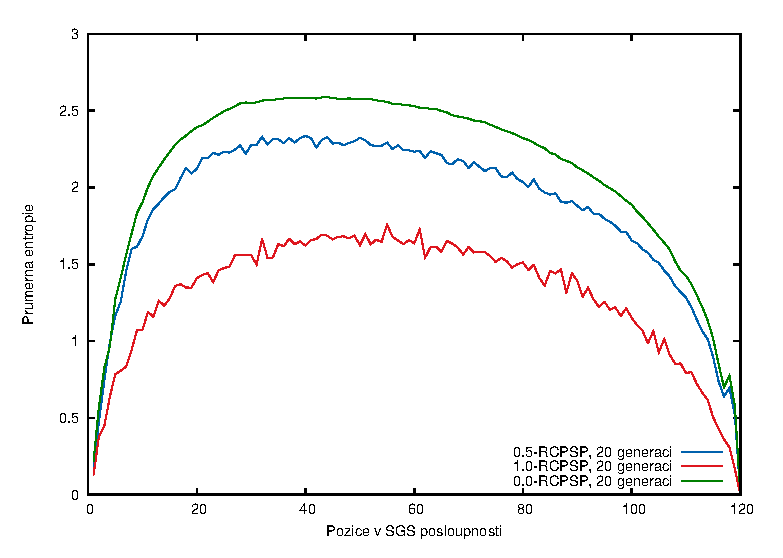
\includegraphics[width=0.9\textwidth]{img/ent.eps}
  \caption{Průměrná entropie pravděpodobnostního rozdělení pro 20 generací. Výsledky tvarem odpovídají výsledkům
  v \cite{Merkle00antcolony, 1027745} pro 250 generací.  Z provedeného experimentu vyplývá (podobně jak v \cite{Merkle00antcolony, 1027745}), 
  že entropie, která odpovídá výběru aktivity doprostřed SGS seznamu, má vyšší hodnotu než entropie odpovídající výběru aktivity do
  okrajových pozic SGS seznamu. Prostředním pozicím totiž odpovídá větší množina vhodných aktivit. Z grafu také vyplývá, že pro 
  hodnotu $c = 1.0$ je průměrná entropie menší než entropie pro parametry $c = 0.5$ a $c = 0.0$.}
  \label{img:ent}
\end{figure}

\subsection{Experiment 4 -- Hledání opt. parametrů pro sadu j30}
Poslední provedený experiment, který již nebyl proveden v \cite{Merkle00antcolony, 1027745} má za cíl najít optimální parametry $c$ a $\rho$ pro 
testovací sadu j30. Instance této testovací sady obsahují 30 aktivit. Kromě nalezení opt. parametrů je také zkoumán vliv 
lokální optimalizační strategie. Parametry
první části experimentu byly zvoleny následovně: velikost populace mravenců $m = 5$, $\rho = 0.025$, $p_w = 0.01$ a 100
generací. Výsledky experimentu
jsou uvedeny na obr.~\ref{img:j30}.

\begin{figure}[!ht]
  \centering
  \includegraphics[height=10cm]{img/j30.eps}
  \caption{Výsledky experimentu nad testovací sadou j30 -- procentuální odchylka od makespanu optimálního řešení pro různé hodnoty $c$.
    Výsledky jsou zprůměrovány přes všech více než 450 instancí v sadě j30.
    Cílem bylo zjistit vliv parametru $c$ na kvalitu řešení. Z grafu vyplývá, že
     pro $c$-RCPSP-LO se 100 provedenými generacemi bylo nejlepších výsledků dosaženo pro parametr $c = 0.5$. Taktéž se 
     ukázal velký vliv lokální optimalizace a počtu generací na kvalitu nalazených řešení. V případě $c$-RCPSP-LO s 20 generacemi se pro každý problém provedla 
     lokální optimalizace pouze jedenkrát a i přesto jsme dosáhli mnohem lepších výsledků než pro $c$-RCPSP se stejným počtem generací.}
  \label{img:j30}
\end{figure}

V dalším navazujícím experimentu se pokusím určit nejvýhodnější parametr $\rho$ pro nejlepší výsledek z minulého experimentu, tedy pro
0.5-RCPSP-LO. Experiment je proveden se stejnými parametry jako v předchozí části a stejný počet (100) generací nad testovací sadou j30. 
Výsledky experimentu jsou uvedeny v tabulce~\ref{tab:j30rho}. 

\begin{table}[ht!]
  \catcode`\-=12
\begin{center}
  \begin{tabular}{ | c | c | }
    \hline
    \multicolumn{2}{|c|}{$0.5$\textbf{-RCPSP-LO}} \\
    \hline
    $\rho$ & Odchylka od optimálního řešení [\%] \\ \hline
    0.002 & 0.82 \\ \hline
    0.025 & 0.73 \\ \hline
    0.2 & 0.68 \\ \hline
    0.6 & 1.10 \\ \hline
  \end{tabular}
\end{center}
\caption{Výsledky části experimentu 4. Hodnoty odchylek od optimálního řešení jsou zprůměrovány 
přes všechny instance testovací sady j30. Z experimentů plyne, že pro parametr $c = 0.5$ a 100 generací je
pro získání nejlepších výsledků vhodné zvolit poměrně vysokou hodnotu $\rho$ (konkrétně $\rho = 0.2$). Ne ale příliž 
velkou, protože již pro $\rho = 0.6$ dostáváme podstatně horší výsledky, které jsou srovnatelné pro $c$-RCPSP (nepoužije se lokální optimalizační strategie)
pro 100 generací a $\rho = 0.025$ (z předchozí části experimentu).}
\label{tab:j30rho}
\end{table}

\subsection{Závěr experimentů}
Celkem byly provedeny 4 experimenty, které zkoumaly různé aspekty implementované metody pro řešení RCPSP. 
Nejprve byla zkoumána odchylka od dolního ohraničení kritické cesty pro různé hodnoty parametru $c$
a rovněž odchylka od dosud nejlepších známých řešení. V dalším experimentu byla zkoumána průměrná entropie
pro různé hodnoty $c$ a také vliv parametru $\rho$ na kvalitu řešení.


\section{Závěr}
Tato práce se věnovala řešení RCPSP s využitím optimalizace pomocí kolonie mravenců. V rámci práce vznikl nástroj, který 
implementuje algoritmus popsaný v \cite{Merkle00antcolony, 1027745}, pro řešení RCPSP. Nástroj je implementován v jazyce 
Python a obsahuje i některé heuristiky
popsané v těchto článcích -- lokální optimalizační strategie, kombinace přímého a souhrnného vyhodnocení a zapomínání 
nejlepších řešení. Některé heuristiky popsané v \cite{1027745} např. obousměrné prohledávání implementováno nebylo. S tímto
nástrojem byly provedeny experimenty (které byly také provedeny v \cite{Merkle00antcolony, 1027745}), které měli za cíl 
ověřit úspěšnost metody a zjistit vliv některých parametrů na kvalitu řešení. Z provedených experimentů vyplývá, že je 
nejvýhodnější zvolit parametr $c = 0.5$ a větší hodnotu $\rho$ pro menší počet generací. Kvůli výpočetní náročnosti musely být
experimenty provedeny s menším počtem generací než je uvedeno v článcích, proto je v této práci dosaženo horších
výsledků než v \cite{Merkle00antcolony, 1027745}.  I přes to se pomocí vytvořeného nástroje pro testovací sadu j120 
knihovny PSPLIB podařilo pro 100 generací s lok. opt. strategií dosáhnout nejlepšího známého řešení v pětině případů.

\newpage
\appendix
\section{Manuál k programu}
Program se spouští pomocí příkazu \texttt{python} s hlavním souborem \texttt{rcpsp.py}. Parametry
programu jsou: cesta k souboru, který obsahuje definici instance RCPSP (ve formátu, který je používán
v knihovně PSPLIB, soubor s příponou .sm) a počet aktivit v projektu (bez aktivity zahájení a ukončení projektu). 
Tedy například: 
\begin{center}
\texttt{python rcpsp.py j1201\_1.sm 120}
\end{center}
Parametry programu lze nastavit v souboru \texttt{rcpsp.py}. Výstupem programu je potom makespan nejlepšího nalezeného řešení. 

\bibliographystyle{czplain}
\bibliography{literatura}{}

\end{document}